\documentclass{article}
\usepackage[utf8]{inputenc}

\usepackage{graphicx}
\graphicspath{{images/}}

\usepackage{caption}
\usepackage{subcaption}
\captionsetup{compatibility=false}

\title{Polytope}
\author{OfficialURL, }
\date{February 2021}

\begin{document}

\maketitle

\section{Introduction}
Welcome to the Polytope Discord! Here we discuss Polytopes, which is a general term that encompasses polygons (2D), polyhedra (3D), polychora (4D), and so on for any dimension.

\section{Regular polytopes}
There are multiple definitions for when a polytope is \textit{regular}, but they all require every element (vertices, edges, faces, etc.) to ``look the same.''

\section{Uniform polytopes}
Intuitively, a polytope is \textit{uniform} when all of its facets are regular and all of its vertices ``look the same.'' To see what we mean, let's look at a few examples.

\begin{figure}[h]
\centering
\begin{subfigure}{.33333\textwidth}
  \centering
  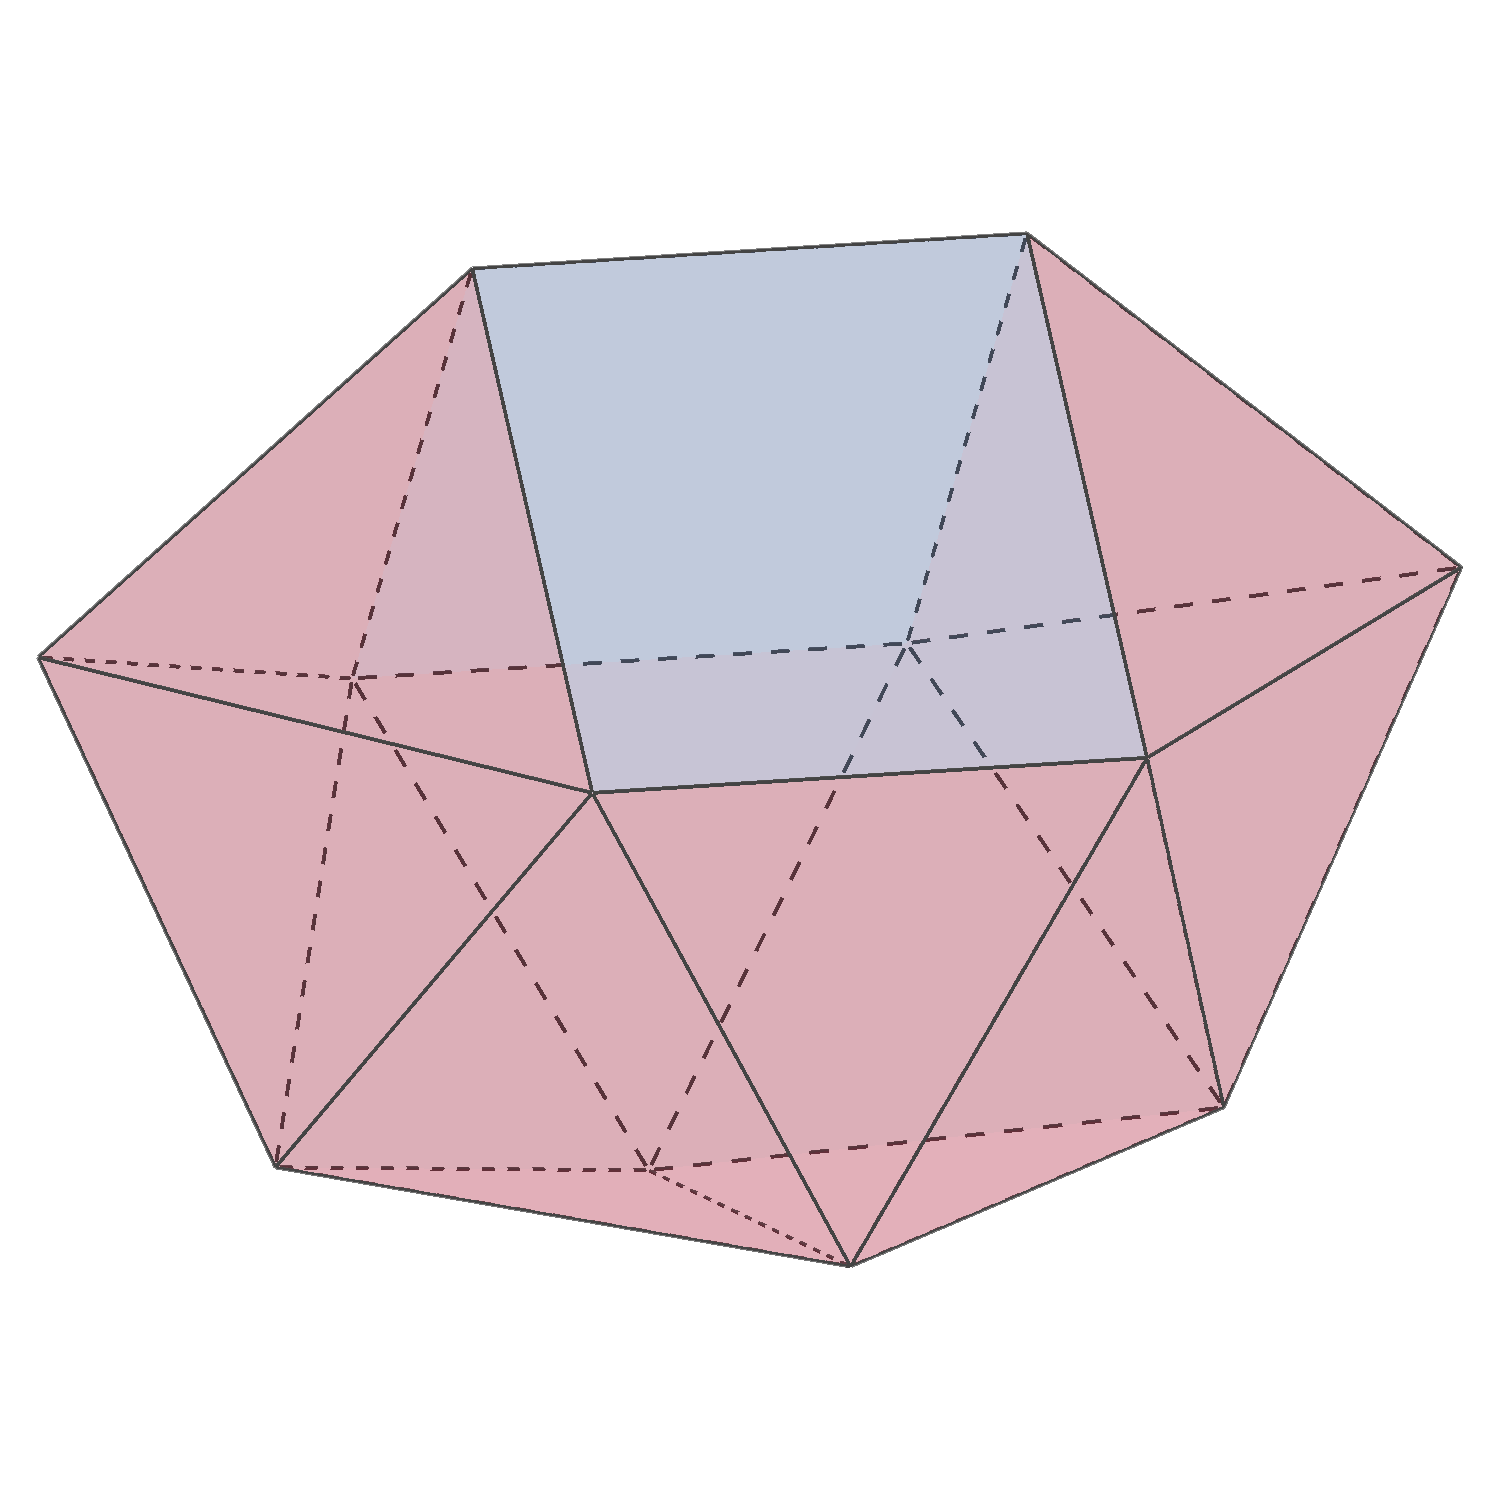
\includegraphics[width=.5\linewidth]{Sphenomegacorona}
  \caption{Sphenomegacorona}
  \label{fig:polyhedra_1}
\end{subfigure}%
\begin{subfigure}{.33333\textwidth}
  \centering
  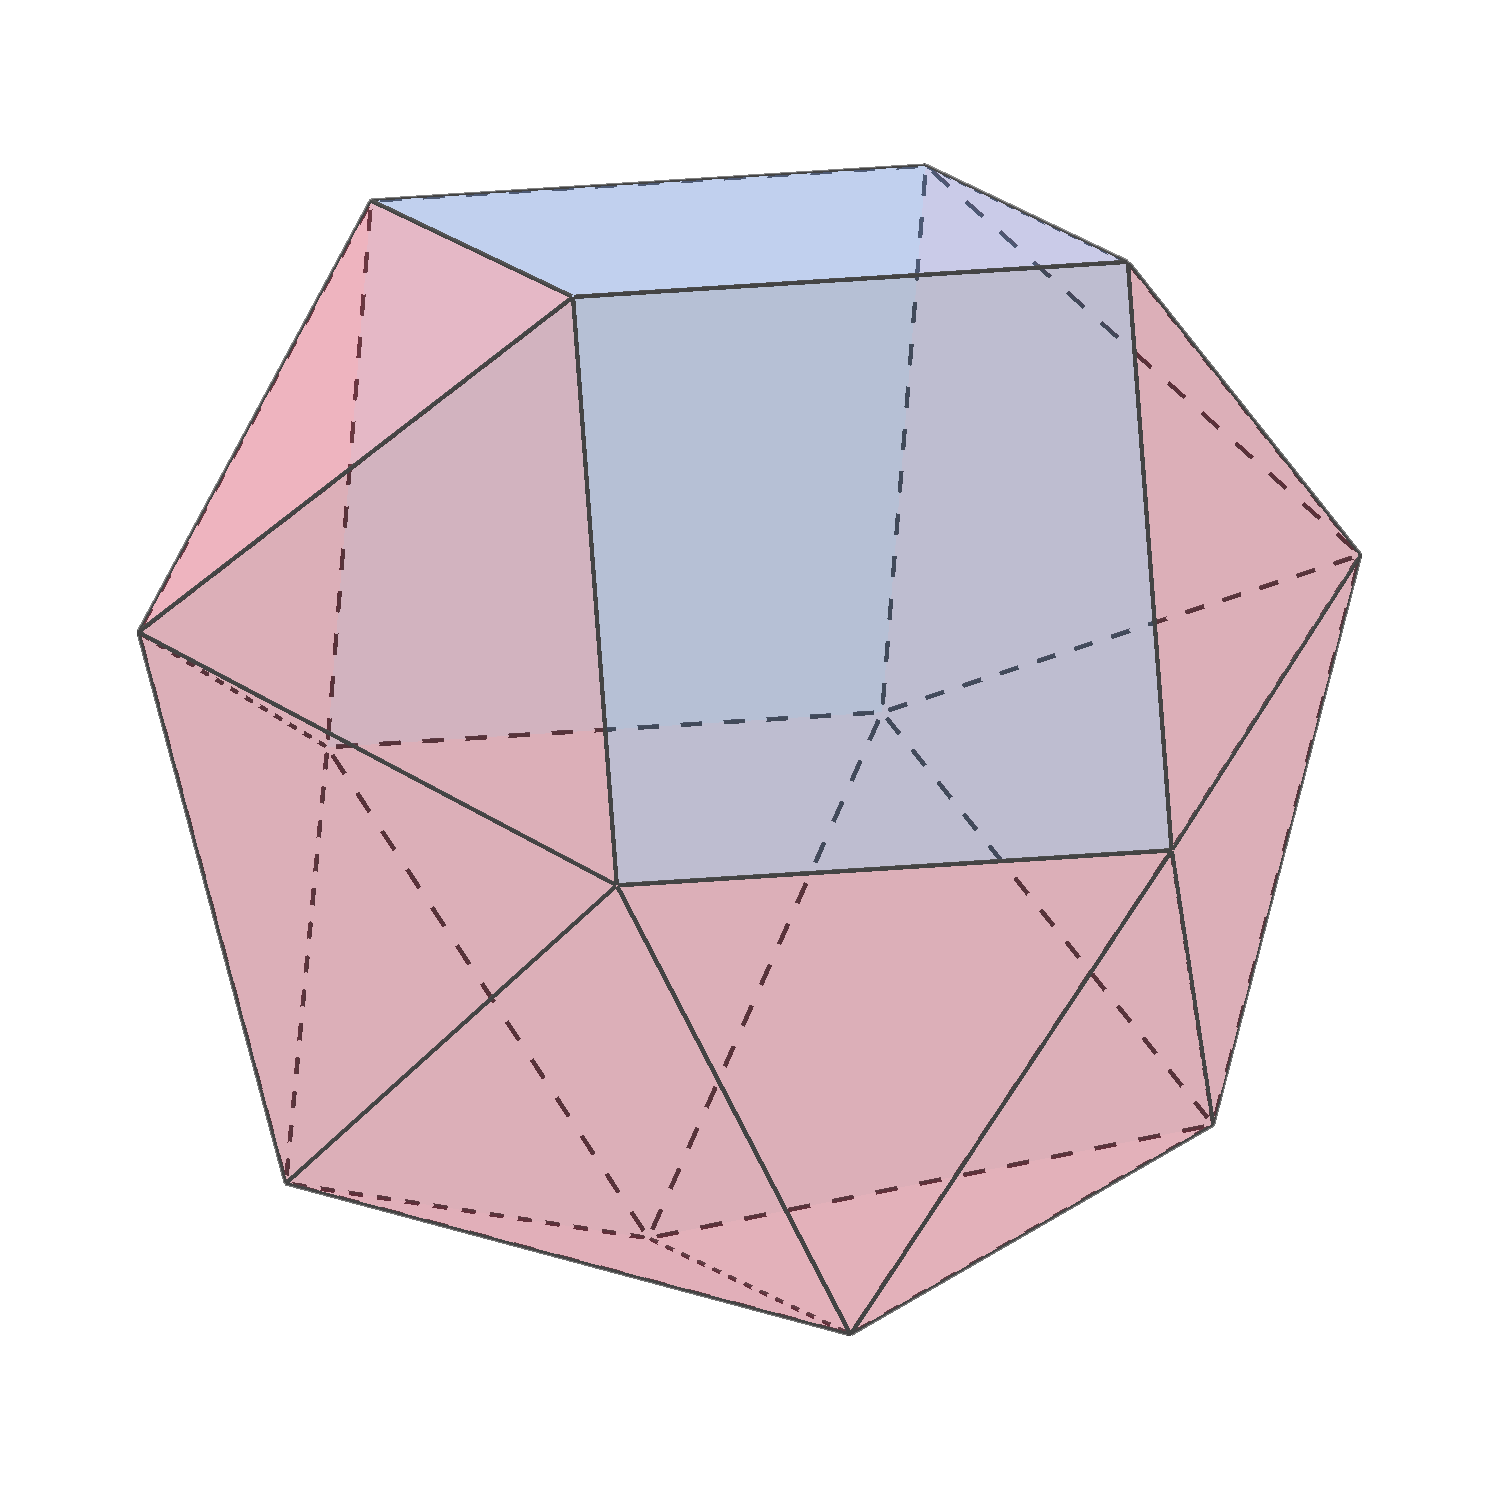
\includegraphics[width=.5\linewidth]{Hebesphenomegacorona}
  \caption{Hebesphenomegacorona}
  \label{fig:polyhedra_2}
\end{subfigure}%
\begin{subfigure}{.33333\textwidth}
  \centering
  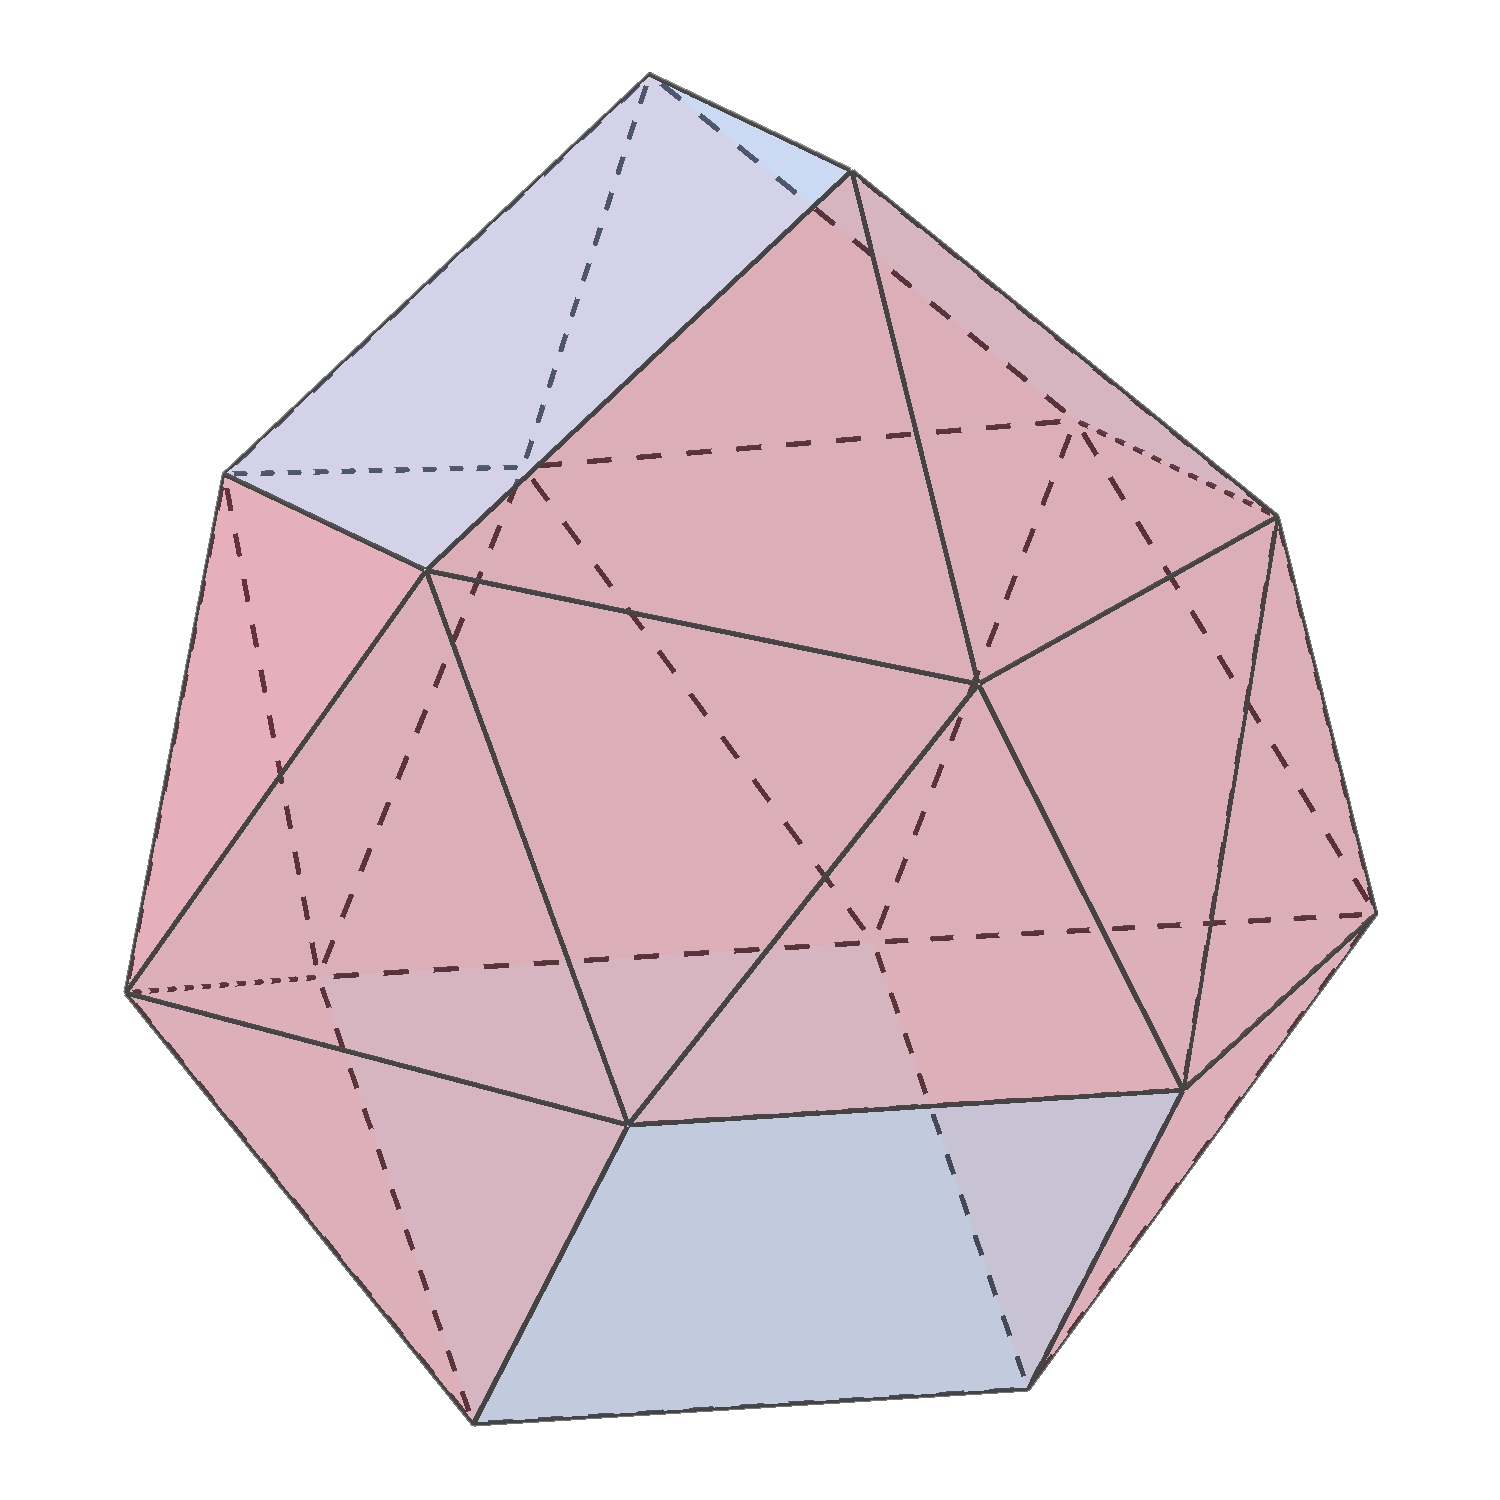
\includegraphics[width=.5\linewidth]{Disphenocingulum}
  \caption{Disphenocingulum}
  \label{fig:polyhedra_3}
\end{subfigure}%
\caption{Test images!}
\label{fig:polyhedra}
\end{figure}


\end{document}
